\documentclass[12pt,a4paper]{article}

\usepackage[utf8]{inputenc}
\usepackage[T2A]{fontenc}
\usepackage[english,russian]{babel}
\usepackage{amsmath}
\usepackage{listings}
\usepackage{caption}

\usepackage{amsmath,amsfonts,amssymb,amsthm,mathtools}

\usepackage{graphicx}
\usepackage{float}
\usepackage{wrapfig}


\author{\textit{Выполнил: Кутепов Никита, РК6-55Б}}
\title{\textit{Задача 5.2}}
\date{}

\begin{document}

\maketitle

\newpage
\section*{Задание}
Требуется найти численное решение задачи Коши с помощью метода Эйлера, используя шаг $h = 0.5$:

\begin{equation*}
	\frac{dy}{dt} = \alpha e^{\beta (t-y)},
	y(0) = 1, 
	t \in [0;1],
\end{equation*}
где $\alpha = 0.5$, $\beta = 1$.

Дополнительно требуется найти точное решение указанной задачи Коши, продемонстрировать графики численного и точного решений на одной координатной плоскости, а также сравнить полученные абсолютные погрешности вычислений с верхней границей глобальной погрешности метода Эйлера.
\section*{Решение}

Рассмотрим следующее ОДУ:

\begin{equation}
	\frac{dy}{dt} = \alpha e^{\beta (t-y)},
\end{equation}
где $t \in [0;1]$, $y(0) = 1$.

Запишем формулировку метода Эйлера [1]:
\begin{equation}\label{1}
	w_0 = \alpha,
\end{equation}
\begin{equation}\label{2}
	w_{i+1} = w_i + h  f(t_i, w_i), 
	i = 0,1...,m-1,
\end{equation}
при этом ожидаем, что $w_i \approx y(t_i)$, а $t_i = a + ih$, $i = 0,1,...,m$.

Учитывая, что $h = 0.5$ и $m = \frac{b - a}{h} = 2$, перепишем (\ref{1}) и (\ref{2}):
\begin{equation}\label{3}
	y(t_0) \approx w_0 = 1, t_0 = 0,
\end{equation}
\begin{equation}\label{3}
	y(t_1) \approx w_1 = w_0 + hf(t_0, w_0) = 1 + 0.5 \cdot 0.5 \cdot e^{(0 - 1)} \approx 1.093, t_1 = 0.5,
\end{equation}
\begin{equation}\label{3}
	y(t_2) \approx w_2 = w_1 + hf(t_1, w_1) = 1.093 + 0.5 \cdot 0.5 \cdot e^{(0.5 - 1.093)} \approx 1.232, t_2 = 1,
\end{equation}

В итоге получаем численное решение задачи Коши с помощью метода Эйлера:
\begin{equation}\label{3}
	{\{t_i,y_i\}}^{m=2}_{i=0}: (t_0,y_0) = (0,1), (t_1,y_1) = (0.5,1.093), (t_2,y_2) = (1,1.232).
\end{equation}

Теперь найдем точное решение задачи Коши:
\begin{equation}
	\frac{dy}{dt} = 0.5 e^{(t-y)},
\end{equation}
\begin{equation}
	2e^{y(t)} dy(t)  = e^t dt,
\end{equation}
\begin{equation}
	\int 2e^{y(t)} dy(t) \frac{dt}{dt}  = \int e^t dt,
\end{equation}
\begin{equation}
	2e^{y(t)} = e^t + C_1	
\end{equation}
\begin{equation}
	y(t) = ln(0.5(e^t + C_1))	
\end{equation}

Так как $y(0) = 1$, $C_1 = -1 + 2e$.
\begin{equation}
	y(t) = ln(0.5(e^t + C_1))	
\end{equation}
Тогда точное решение задачи Коши:
\begin{equation}
	y(t) = ln(0.5(e^t - 1 + 2e))	
\end{equation}

Выполним построение точного и численного решений задачи Коши, используя скрипт, написанный на языке программирования Python. 

\begin{lstlisting}[language=Python, caption={Построение графиков точного и численного решений задачи Коши.}]
import math
import numpy as np
import matplotlib.pyplot as plt


def f(t, y):
    return 0.5 * math.e ** (t - y)


def y_solution(t):
    return math.log(0.5 * (math.e ** t - 1 + 2 * math.e))


def time_integrate(y_0, a, b, h):
    m = int((b - a) / h)
    y = np.zeros((m + 1,))
    t = np.linspace(a, b, m + 1)
    y[0] = y_0

    for i in range(m):
        t_i = a + i * h
        y[i + 1] = y[i] + h * f(t_i, y[i])

    return t, y


if __name__ == '__main__':
    y_0 = 1
    a = 0
    b = 1
    h = 0.5
    t_approx, y_approx = time_integrate(y_0, a, b, h)
    t = np.linspace(a, b, 200)
    fig, ax = plt.subplots(1, 1, figsize=(14, 6))
    y = [y_solution(i) for i in t]
    ax.plot(t, y, '-', linewidth=2, label=r"$y(t)$")
    ax.plot(t_approx, y_approx, 'o--', linewidth=2, label=r"$w_i$")
    ax.set_xlabel(r'$t$', fontsize=16)
    ax.set_ylabel(r'$y$', fontsize=16)
    ax.grid()
    ax.legend(loc='lower right', fontsize=16)
    plt.show()

\end{lstlisting}

Построим графики точного и численного решений задачи Коши.
\begin{figure}[h]
	\center{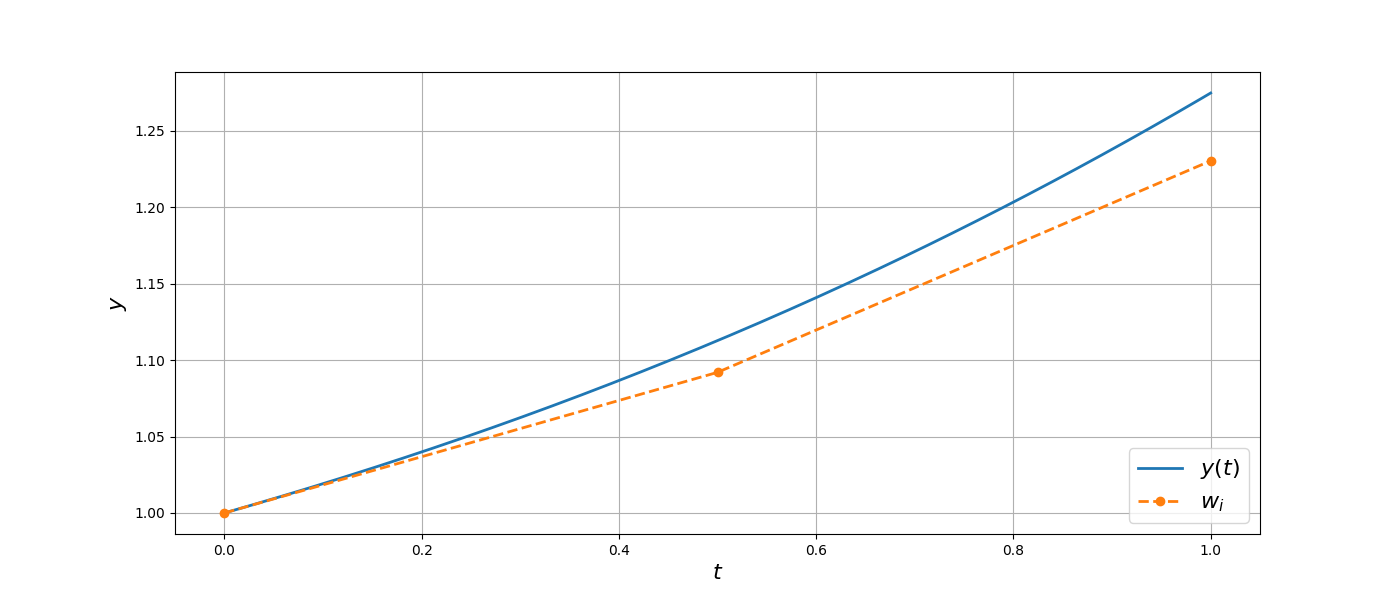
\includegraphics[scale=0.4]{sem_6.png}}
	\caption{Графики точного и численного решений задачи Коши.}
	\label{fig:image}
\end{figure}

Программно вычислим абсолютную погрешность в узлах: $t_0 = 0$, $t_1 = 0.5$, $t_2 = 1$:
\begin{equation}
	(0, 1): \delta_0 = 0 	
\end{equation}
\begin{equation}
	(0.5, 1.093): \delta_1 \approx 0.021	
\end{equation}
\begin{equation}
	(1, 1.232): \delta_2 \approx 0.044	
\end{equation}


Теперь мы можем приступить к рассмотрению теоремы о верхней границе глобальной
погрешности метода Эйлера.

\begin{equation}
	\left| y(t_i) - w_i  \right| \leq \frac{hM}{2L}(e^{L(t_i - a)} - 1), i=0,1,..,m, 
\end{equation}
где $h = \frac{b - a}{m}$, L - константа Липшица, $M > max|f^{''}(t)|$

Сравним полученные абсолютные погрешности вычислений с верхней границей глобальной погрешности, для этого найдем максимальное значение второй производной функции $y(t)$ на участке [0;1]:
\begin{equation}\label{diff_1}
	y^{'}(t) = \frac{e^t}{(e^t - 1)+2e}
\end{equation}
\begin{equation}
	y^{''}(t) = \frac{(1 - \frac{e^t}{e^t - 1 + 2e})e^t}{e^t - 1 + 2e}
\end{equation}

Построим график данной функции, чтобы найти максимальное значение на заданном интервале:
\begin{figure}[h]
	\center{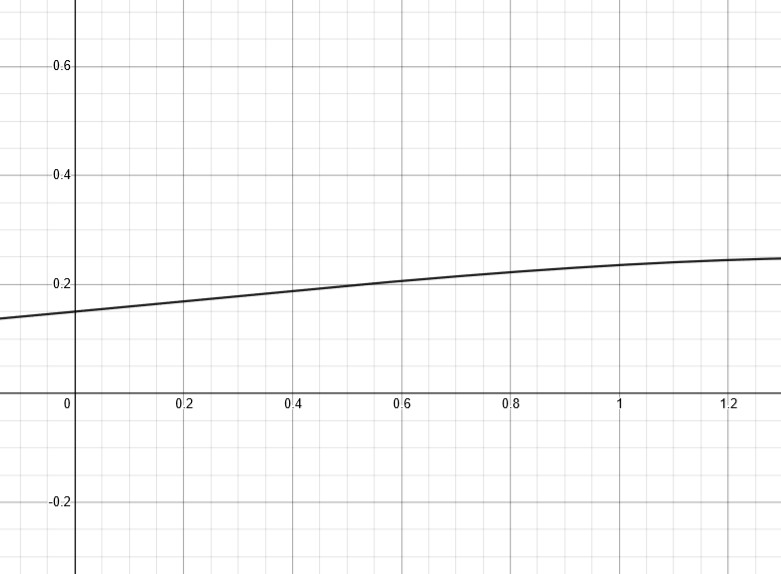
\includegraphics[scale=0.4]{sem_6_1.jpg}}
	\caption{График второй производной функции y(t).}
	\label{fig:image}
\end{figure}

Из графика видно, что максимальное значение функция принимает в точке t=1:
\begin{equation}
	y^{''}(1) \approx 0.2356
\end{equation}
Тогда M = 0.236, найдем константу Липшица по формуле:
\begin{equation}
	L = max|f^{'}(t)|	
\end{equation}


Воспользуемся (\ref{diff_1}), чтобы найти максимальное значение производной на участке [0;1], рассмотрим график первой производной:
\begin{figure}[h]
	\center{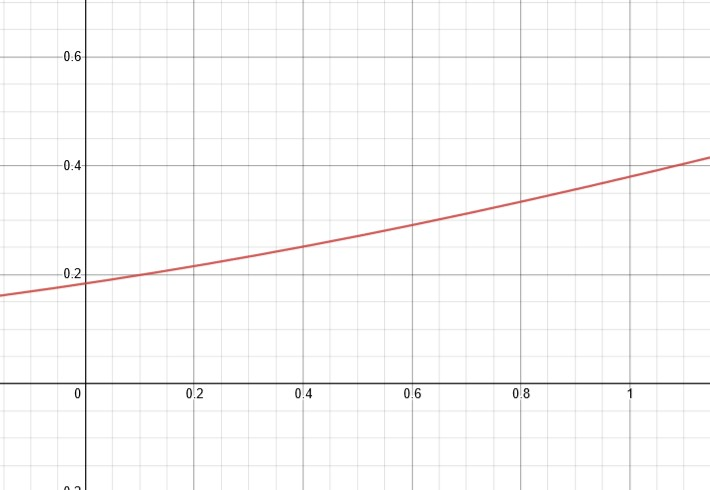
\includegraphics[scale=0.4]{sem_6_2.jpg}}
	\caption{График первой производной функции y(t).}
	\label{fig:image}
\end{figure}


Заметим, что максимальное значение функция принимает в точке t=1:
\begin{equation}
	L = f^{'}(1) \approx 0.3799
\end{equation}

Теперь, зная L и M, сравним полученные абсолютные погрешности с верхней границей глобальной погрешности:
\begin{equation}
	t_0: \left |  y_0 - w_0 \right | \leq \frac{hM}{2L} (e^{(t_{0} - a)L} - 1) =  0, \bigtriangleup_0 = 0 - \delta_0 = 0
\end{equation}
\begin{equation}
	t_1: \left |  y_1 - w_1 \right | \leq \frac{hM}{2L} (e^{(t_{1} - a)L} - 1) \approx 0.032, \bigtriangleup_1 = 0.032 - \delta_1 = 0.011  
\end{equation}
\begin{equation}
	t_2: \left |  y_2 - w_2 \right | \leq \frac{hM}{2L} (e^{(t_{2} - a)L} - 1) \approx 0.072, \bigtriangleup_2 = 0.072 - \delta_2 = 0.028
\end{equation}
\subsubsection*{Список использованных источников}

\begin{enumerate}
	\item Першин А.Ю. Лекции по курсу "Вычислительная математика". Москва, 2018-2021. Тема "Численное решение задачи Коши для систем ОДУ"
\end{enumerate}
\end{document}
